
To ensure that the combination of higher-order discretization schemes remains an unconditionally stable time-marching method, we perform Fourier analysis (also known as Von Neumann stability analysis)~\cite{leveque2007finite}.
A time marching scheme
\begin{equation}
    \Psi_{k+1/2} = \bm{K} \Psi_{k-1/2} \;,
\end{equation}
where $\bm{K}$ is the time iteration matrix, is unconditionally stable when the Von Neumann stability condition is met:
\begin{equation}
    \sup(|\lambda_{K}|) \leq 1 \;,
    \label{eq:unconstab}
\end{equation}
where $\lambda_K$ are the eigenvalues of $\bm{K}$ \cite{golub_matrix_1983, isaacson_numerical_1966}.
$\bm{K}$ can be derived for a given model problem.
We consider a model problem consisting of a homogeneous infinite medium with no scattering to derive the eigenfunction of the time-dependent multiple balance, simple corner balance discretization scheme.
Since this problem has no scattering, each angle can be solved independently of every other angle, and no operator splitting is required.
We first start by describing the absolute error of the angular flux at time step $(k+1/2)$:
\begin{equation}
    \mathbf{f}_{k+1/2} = \Psi_{\text{exact}} - \Psi_{k+1/2} \;.
\end{equation}
Then, we define a Fourier ansätz for the error propagated through a time step:
\begin{subequations}
\begin{align}
    f_{k+1/2,j,L} &= \lambda^{k+1}a_t e^{i\omega j} \; ,
    &
    f_{k+1/2,j,R} &= \lambda^{k+1}b_t e^{i\omega j} \; ,
\end{align}
\begin{align}
    f_{k,j,L} &= \lambda^{k}c_t e^{i\omega j} \; ,
    &
    f_{k,j,R} &= \lambda^{k}d_t e^{i\omega j} \; ,
\end{align}
\begin{align}
    f_{k-1/2,j,L} &= \lambda^{k}a_t e^{i\omega j} \; ,
    &
    f_{k-1/2,j,R} &= \lambda^{k}b_t e^{i\omega j} \; ,
\end{align}
\end{subequations}
where $k$ is the time step, $i=\sqrt{-1}$, $\lambda$ is the eigenvalue, $\omega$ is the wave number, $j$ is cell index and $a_t$, $b_t$, $c_t$, and $d_t$ are components of the eigenvector.
Substituting our ansätz into the error form of Eqs.~\eqref{eq:scb-mb} and assuming $\mu>0$, we simplify to form:
\begin{subequations}
\begin{equation}
    \label{eq:eig1}
    \frac{\Delta x}{2} \frac{1}{v \Delta t} (\lambda a_t- a_t) + \mu \left(\frac{c_t+d_t}{2} - d_t e ^{-i\omega} \right) + \frac{\Sigma\Delta x }{2}c_t = 0 \; ,
\end{equation}
\begin{equation}
\label{eq:eig2}
    \frac{\Delta x}{2} \frac{1}{v \Delta t} (\lambda b_t - b_t) + \mu \left( c_te^{i\omega} - \frac{c_t+d_t}{2} \right) + \frac{\Sigma\Delta x }{2}d_t = 0 \; ,
\end{equation}
\begin{equation}
\label{eq:eig3}
    \frac{\Delta x}{2} \frac{2}{v \Delta t} (\lambda a_t - c_t) + \lambda\mu \left( \frac{a_t+b_t}{2} - b_t e^{-i\omega} \right) + \frac{\Sigma\Delta x }{2}a_t \lambda = 0 \; ,
\end{equation}
\begin{equation}
\label{eq:eig4}
    \frac{\Delta x}{2} \frac{2}{v \Delta t} (\lambda b_t - d_t) + \lambda\mu \left( d_t e^{i\omega} + \frac{c_t+d_t}{2} \right) + \frac{\Sigma\Delta x}{2} b_t\lambda = 0 \;,
\end{equation}
\end{subequations}
combining Eq.~\eqref{eq:eig1} into \eqref{eq:eig2}:
\begin{equation}
    \label{eq:f_a-1}
    \begin{bmatrix}
        c_t\\d_t
    \end{bmatrix}
    = \bm{K_{+}}^{-1} \frac{\Delta x}{2}\frac{1}{v\Delta t}(1-\lambda)
    \begin{bmatrix}
        a_t\\b_t
    \end{bmatrix} \;,
\end{equation}
where
\begin{equation}
    {\bm{K_{+}}} = 
    \begin{bmatrix}
    \frac{\mu}{2}+\frac{\Sigma \Delta x}{2} & \mu (\frac{1}{2} - e^{-i\omega}) \\
    -\frac{\mu}{2} & \frac{\mu}{2}+\frac{\Sigma \Delta x}{2}
    \end{bmatrix} \;.
\end{equation}
Then, doing the same with Eq.~\eqref{eq:eig3} into \eqref{eq:eig4}:
\begin{equation}
    \label{eq:f_a-2}
    \lambda \left( \bm{K_{+}} + \frac{\Delta x}{v \Delta t} \bm{I} \right)  \begin{bmatrix}
        a_t \\ b_t
    \end{bmatrix} = \frac{\Delta x}{v\Delta t} \begin{bmatrix}
        c_t \\ d_t
\end{bmatrix} \; ,
\end{equation}
where $\bm{I}$ is the identity matrix. Combining Eq.~\eqref{eq:f_a-1} into \eqref{eq:f_a-2} gives
\begin{equation}
    \lambda
    \begin{bmatrix}
        a_t \\b_t
    \end{bmatrix}
    = \left[ \bm{K_{+}} + \frac{\Delta x}{v\Delta t} \bm{I} + \gamma\bm{K_{+}}^{-1} \right]^{-1} \gamma \bm{K_{+}}^{-1}
    \begin{bmatrix}
        a_t \\ b_t
    \end{bmatrix} \; ,
\end{equation}
where $\gamma = \frac{\Delta x}{v\Delta t}  \frac{\Delta x}{2v\Delta t}$.
This can then be more appropriately posed as an eigenfunction:
\begin{equation}
    \lambda_K
    \bm{a}
    = \bm{K} \bm{a}\;,
\end{equation}
where
\begin{equation}
    \bm{K} = \gamma \left( \bm{K_{+}}\bm{K_{+}} + \frac{\Delta x}{v \Delta t}\bm{K_{+}} + \gamma \bm{I}\right)^{-1}
\end{equation}
and the eigenvector is
\begin{equation}
    \bf{a} = \begin{bmatrix}
        a_t, & b_t
    \end{bmatrix} ^T \;.
\end{equation}
The analysis is similar for $\mu<0$ only with
\begin{equation}
    \bm{K_{-}} = \begin{bmatrix}
        -\frac{\mu}{2} + \frac{\Sigma\Delta x}{2} & \frac{\mu}{2} \\
        \mu \left ( e^{i\omega} - \frac{1}{2} \right) & -\frac{\mu}{2} + \frac{\Sigma\Delta x}{2} 
    \end{bmatrix} \;.
\end{equation}

This system can be numerically solved after making discrete selections of $\mu \in [-1, 1]$ and $\omega \in (0,2\pi]$ at a point in the perameter space ($\Delta x$, $\Delta t$, $v$, $\Sigma$) with \texttt{numpy.max(numpy.abs(numpy.linalg.eig(K))}~\cite{harris2020array}.

Figure \ref{fig:mb-scb} shows the absolute value of the maximum eigenvalues of $\bm{K}$ at various points in mean free time ($\tau=\Sigma v\Delta t$) and cellular optical thickness ($\delta=\Sigma\Delta x$) at 75 discrete points $\omega \in (0,2\pi]$ in S$_{16}$.
None of $|\lambda_{max}|$ are above one, which means the Von Neumann stability criterion in Eq. \eqref{eq:unconstab} is satisfied and the combination of the multiple balance time discretization and the simple corner balance scheme is unconditionally stable for this infinite homogeneous medium problem with no scattering.
%While experimenting with this method we did find that, under some conditions, it can produce negative fluxes; however, the negative flux oscillations are critically damped and dissipate with time.

\begin{figure}[htbp]
    \centering
    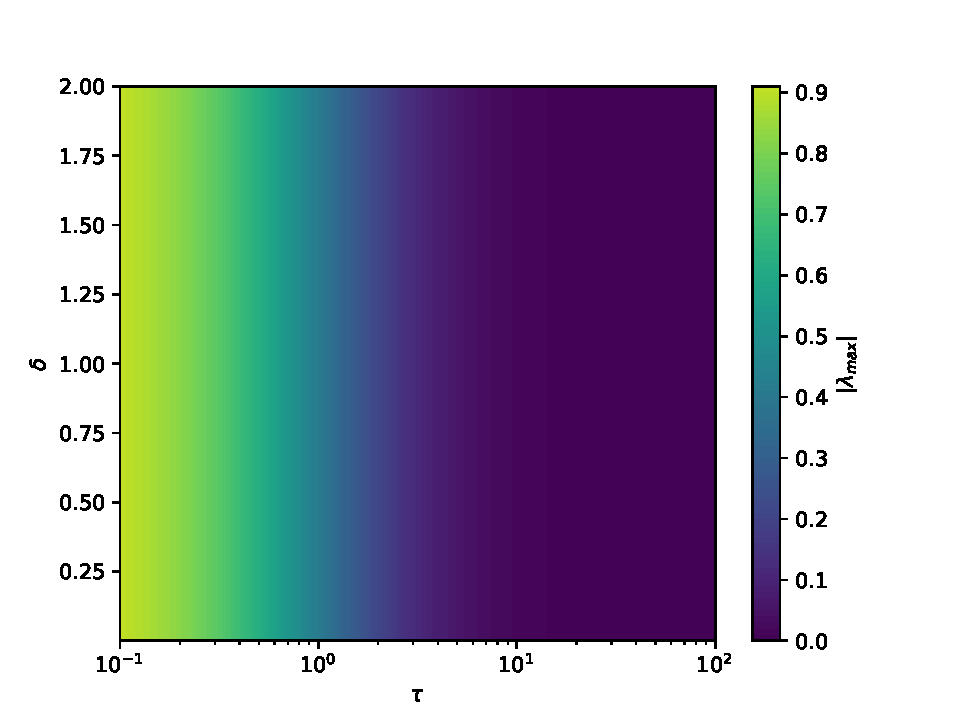
\includegraphics[width=0.75\linewidth]{manuscript2/man2_figs/mb_scb.pdf}
    \caption{$|\lambda_{\max}|$ from numerically solved multiple balance time discretization and simple corner balance Fourier system over choices in mean free time ($\tau$) and cellular optical thickness ($\delta$) in S$_{16}$.}
    \label{fig:mb-scb}
\end{figure}
